\documentclass[1p]{elsarticle_modified}
%\bibliographystyle{elsarticle-num}

%\usepackage[colorlinks]{hyperref}
%\usepackage{abbrmath_seonhwa} %\Abb, \Ascr, \Acal ,\Abf, \Afrak
\usepackage{amsfonts}
\usepackage{amssymb}
\usepackage{amsmath}
\usepackage{amsthm}
\usepackage{scalefnt}
\usepackage{amsbsy}
\usepackage{kotex}
\usepackage{caption}
\usepackage{subfig}
\usepackage{color}
\usepackage{graphicx}
\usepackage{xcolor} %% white, black, red, green, blue, cyan, magenta, yellow
\usepackage{float}
\usepackage{setspace}
\usepackage{hyperref}

\usepackage{tikz}
\usetikzlibrary{arrows}

\usepackage{multirow}
\usepackage{array} % fixed length table
\usepackage{hhline}

%%%%%%%%%%%%%%%%%%%%%
\makeatletter
\renewcommand*\env@matrix[1][\arraystretch]{%
	\edef\arraystretch{#1}%
	\hskip -\arraycolsep
	\let\@ifnextchar\new@ifnextchar
	\array{*\c@MaxMatrixCols c}}
\makeatother %https://tex.stackexchange.com/questions/14071/how-can-i-increase-the-line-spacing-in-a-matrix
%%%%%%%%%%%%%%%

\usepackage[normalem]{ulem}

\newcommand{\msout}[1]{\ifmmode\text{\sout{\ensuremath{#1}}}\else\sout{#1}\fi}
%SOURCE: \msout is \stkout macro in https://tex.stackexchange.com/questions/20609/strikeout-in-math-mode

\newcommand{\cancel}[1]{
	\ifmmode
	{\color{red}\msout{#1}}
	\else
	{\color{red}\sout{#1}}
	\fi
}

\newcommand{\add}[1]{
	{\color{blue}\uwave{#1}}
}

\newcommand{\replace}[2]{
	\ifmmode
	{\color{red}\msout{#1}}{\color{blue}\uwave{#2}}
	\else
	{\color{red}\sout{#1}}{\color{blue}\uwave{#2}}
	\fi
}

\newcommand{\Sol}{\mathcal{S}} %segment
\newcommand{\D}{D} %diagram
\newcommand{\A}{\mathcal{A}} %arc


%%%%%%%%%%%%%%%%%%%%%%%%%%%%%5 test

\def\sl{\operatorname{\textup{SL}}(2,\Cbb)}
\def\psl{\operatorname{\textup{PSL}}(2,\Cbb)}
\def\quan{\mkern 1mu \triangleright \mkern 1mu}

\theoremstyle{definition}
\newtheorem{thm}{Theorem}[section]
\newtheorem{prop}[thm]{Proposition}
\newtheorem{lem}[thm]{Lemma}
\newtheorem{ques}[thm]{Question}
\newtheorem{cor}[thm]{Corollary}
\newtheorem{defn}[thm]{Definition}
\newtheorem{exam}[thm]{Example}
\newtheorem{rmk}[thm]{Remark}
\newtheorem{alg}[thm]{Algorithm}

\newcommand{\I}{\sqrt{-1}}
\begin{document}

%\begin{frontmatter}
%
%\title{Boundary parabolic representations of knots up to 8 crossings}
%
%%% Group authors per affiliation:
%\author{Yunhi Cho} 
%\address{Department of Mathematics, University of Seoul, Seoul, Korea}
%\ead{yhcho@uos.ac.kr}
%
%
%\author{Seonhwa Kim} %\fnref{s_kim}}
%\address{Center for Geometry and Physics, Institute for Basic Science, Pohang, 37673, Korea}
%\ead{ryeona17@ibs.re.kr}
%
%\author{Hyuk Kim}
%\address{Department of Mathematical Sciences, Seoul National University, Seoul 08826, Korea}
%\ead{hyukkim@snu.ac.kr}
%
%\author{Seokbeom Yoon}
%\address{Department of Mathematical Sciences, Seoul National University, Seoul, 08826,  Korea}
%\ead{sbyoon15@snu.ac.kr}
%
%\begin{abstract}
%We find all boundary parabolic representation of knots up to 8 crossings.
%
%\end{abstract}
%\begin{keyword}
%    \MSC[2010] 57M25 
%\end{keyword}
%
%\end{frontmatter}

%\linenumbers
%\tableofcontents
%
\newcommand\colored[1]{\textcolor{white}{\rule[-0.35ex]{0.8em}{1.4ex}}\kern-0.8em\color{red} #1}%
%\newcommand\colored[1]{\textcolor{white}{ #1}\kern-2.17ex	\textcolor{white}{ #1}\kern-1.81ex	\textcolor{white}{ #1}\kern-2.15ex\color{red}#1	}

{\Large $\underline{12n_{0608}~(K12n_{0608})}$}

\setlength{\tabcolsep}{10pt}
\renewcommand{\arraystretch}{1.6}
\vspace{1cm}\begin{tabular}{m{100pt}>{\centering\arraybackslash}m{274pt}}
\multirow{5}{120pt}{
	\centering
	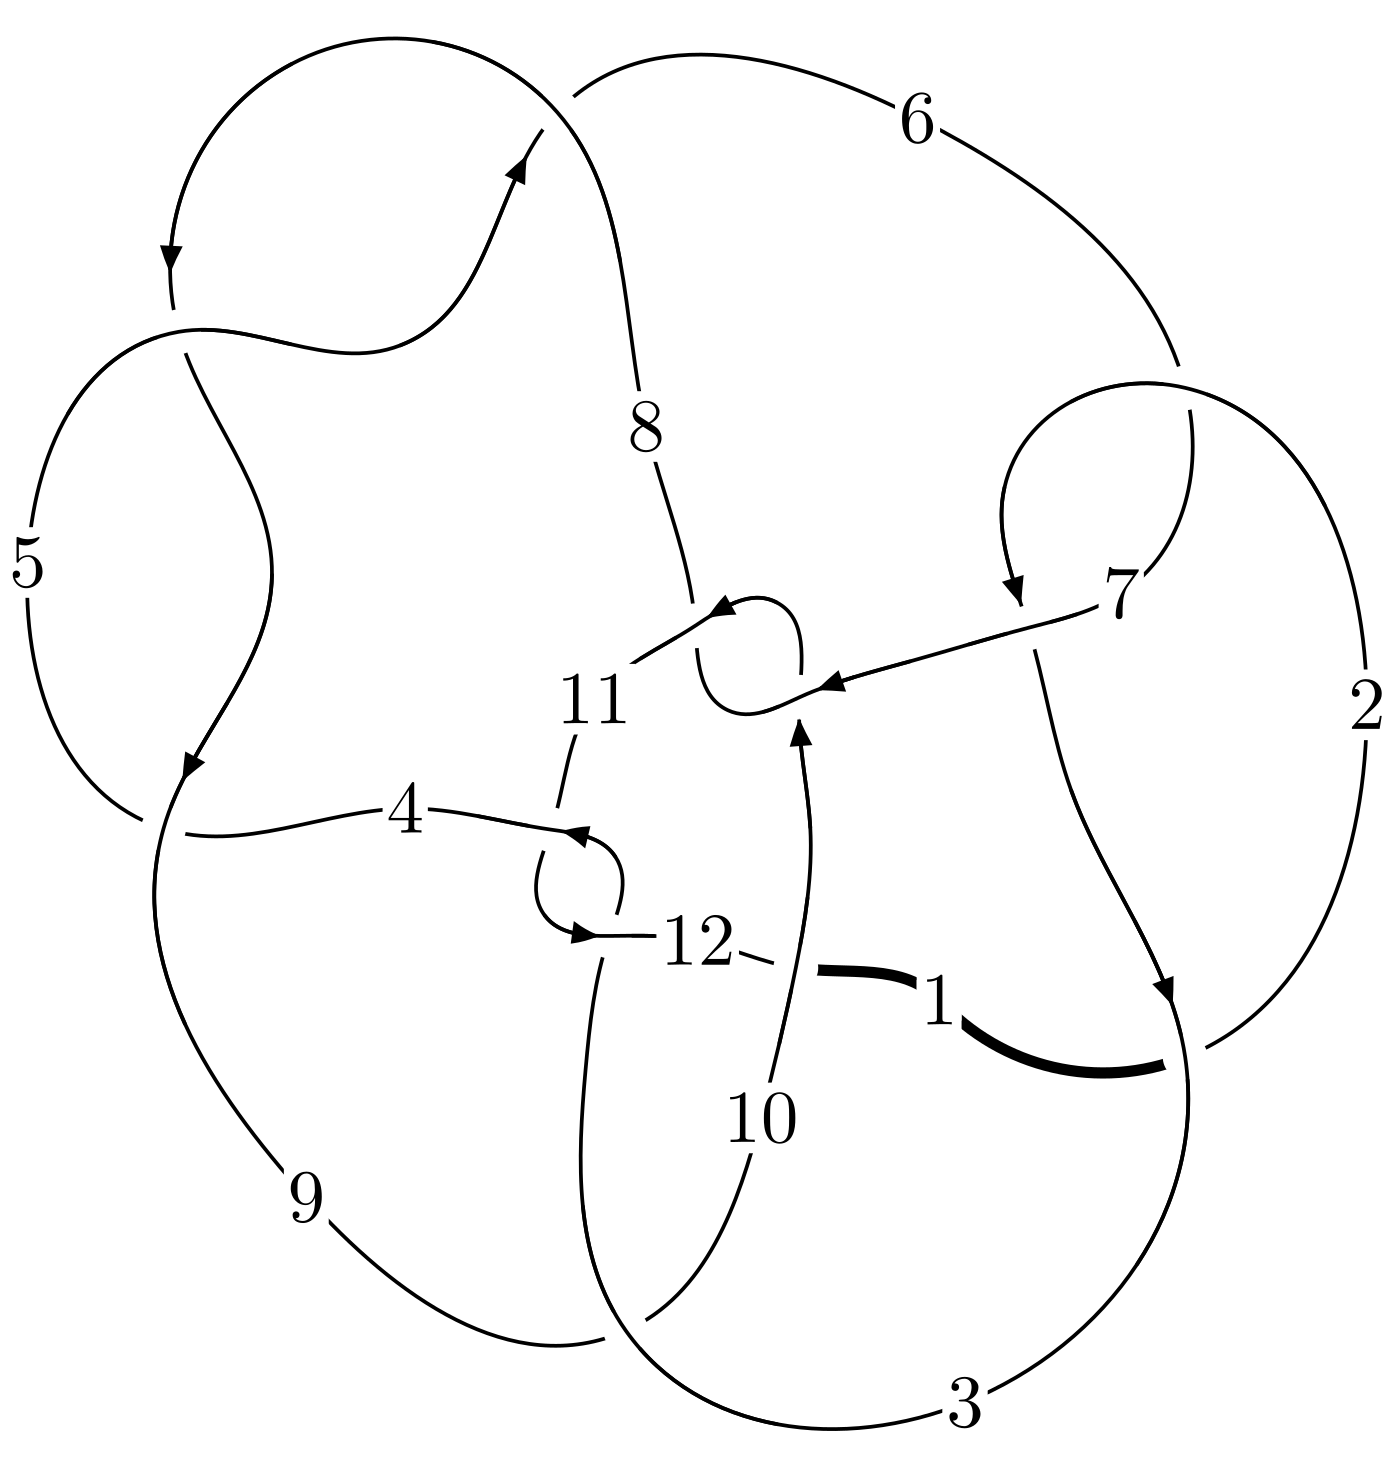
\includegraphics[width=112pt]{../../../GIT/diagram.site/Diagrams/png/2697_12n_0608.png}\\
\ \ \ A knot diagram\footnotemark}&
\allowdisplaybreaks
\textbf{Linearized knot diagam} \\
\cline{2-2}
 &
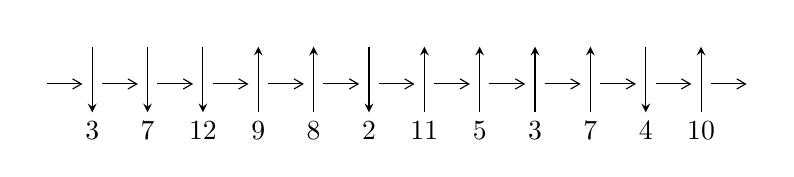
\begin{tikzpicture}[x=20pt, y=17pt]
	% nodes
	\node (C0) at (0, 0) {};
	\node (C1) at (1, 0) {};
	\node (C1U) at (1, +1) {};
	\node (C1D) at (1, -1) {3};

	\node (C2) at (2, 0) {};
	\node (C2U) at (2, +1) {};
	\node (C2D) at (2, -1) {7};

	\node (C3) at (3, 0) {};
	\node (C3U) at (3, +1) {};
	\node (C3D) at (3, -1) {12};

	\node (C4) at (4, 0) {};
	\node (C4U) at (4, +1) {};
	\node (C4D) at (4, -1) {9};

	\node (C5) at (5, 0) {};
	\node (C5U) at (5, +1) {};
	\node (C5D) at (5, -1) {8};

	\node (C6) at (6, 0) {};
	\node (C6U) at (6, +1) {};
	\node (C6D) at (6, -1) {2};

	\node (C7) at (7, 0) {};
	\node (C7U) at (7, +1) {};
	\node (C7D) at (7, -1) {11};

	\node (C8) at (8, 0) {};
	\node (C8U) at (8, +1) {};
	\node (C8D) at (8, -1) {5};

	\node (C9) at (9, 0) {};
	\node (C9U) at (9, +1) {};
	\node (C9D) at (9, -1) {3};

	\node (C10) at (10, 0) {};
	\node (C10U) at (10, +1) {};
	\node (C10D) at (10, -1) {7};

	\node (C11) at (11, 0) {};
	\node (C11U) at (11, +1) {};
	\node (C11D) at (11, -1) {4};

	\node (C12) at (12, 0) {};
	\node (C12U) at (12, +1) {};
	\node (C12D) at (12, -1) {10};
	\node (C13) at (13, 0) {};

	% arrows
	\draw[->,>={angle 60}]
	(C0) edge (C1) (C1) edge (C2) (C2) edge (C3) (C3) edge (C4) (C4) edge (C5) (C5) edge (C6) (C6) edge (C7) (C7) edge (C8) (C8) edge (C9) (C9) edge (C10) (C10) edge (C11) (C11) edge (C12) (C12) edge (C13) ;	\draw[->,>=stealth]
	(C1U) edge (C1D) (C2U) edge (C2D) (C3U) edge (C3D) (C4D) edge (C4U) (C5D) edge (C5U) (C6U) edge (C6D) (C7D) edge (C7U) (C8D) edge (C8U) (C9D) edge (C9U) (C10D) edge (C10U) (C11U) edge (C11D) (C12D) edge (C12U) ;
	\end{tikzpicture} \\
\hhline{~~} \\& 
\textbf{Solving Sequence} \\ \cline{2-2} 
 &
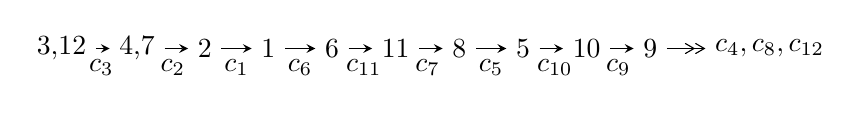
\begin{tikzpicture}[x=23pt, y=7pt]
	% node
	\node (A0) at (-1/8, 0) {3,12};
	\node (A1) at (17/16, 0) {4,7};
	\node (A2) at (17/8, 0) {2};
	\node (A3) at (25/8, 0) {1};
	\node (A4) at (33/8, 0) {6};
	\node (A5) at (41/8, 0) {11};
	\node (A6) at (49/8, 0) {8};
	\node (A7) at (57/8, 0) {5};
	\node (A8) at (65/8, 0) {10};
	\node (A9) at (73/8, 0) {9};
	\node (C1) at (1/2, -1) {$c_{3}$};
	\node (C2) at (13/8, -1) {$c_{2}$};
	\node (C3) at (21/8, -1) {$c_{1}$};
	\node (C4) at (29/8, -1) {$c_{6}$};
	\node (C5) at (37/8, -1) {$c_{11}$};
	\node (C6) at (45/8, -1) {$c_{7}$};
	\node (C7) at (53/8, -1) {$c_{5}$};
	\node (C8) at (61/8, -1) {$c_{10}$};
	\node (C9) at (69/8, -1) {$c_{9}$};
	\node (A10) at (11, 0) {$c_{4},c_{8},c_{12}$};

	% edge
	\draw[->,>=stealth]	
	(A0) edge (A1) (A1) edge (A2) (A2) edge (A3) (A3) edge (A4) (A4) edge (A5) (A5) edge (A6) (A6) edge (A7) (A7) edge (A8) (A8) edge (A9) ;
	\draw[->>,>={angle 60}]	
	(A9) edge (A10);
\end{tikzpicture} \\ 

\end{tabular} \\

\footnotetext{
The image of knot diagram is generated by the software ``\textbf{Draw programme}" developed by Andrew Bartholomew(\url{http://www.layer8.co.uk/maths/draw/index.htm\#Running-draw}), where we modified some parts for our purpose(\url{https://github.com/CATsTAILs/LinksPainter}).
}\phantom \\ \newline 
\centering \textbf{Ideals for irreducible components\footnotemark of $X_{\text{par}}$} 
 
\begin{align*}
I^u_{1}&=\langle 
-4.28549\times10^{26} u^{34}+1.62732\times10^{27} u^{33}+\cdots+1.15843\times10^{27} b+8.44652\times10^{25},\\
\phantom{I^u_{1}}&\phantom{= \langle  }-6.12275\times10^{26} u^{34}+2.45059\times10^{27} u^{33}+\cdots+1.15843\times10^{27} a-1.01126\times10^{28},\\
\phantom{I^u_{1}}&\phantom{= \langle  }u^{35}-4 u^{34}+\cdots+13 u-1\rangle \\
I^u_{2}&=\langle 
- u^8-2 u^7-6 u^6-8 u^5-11 u^4-10 u^3-8 u^2+b-5 u-2,\;-5 u^{14}-15 u^{13}+\cdots+3 a-17,\\
\phantom{I^u_{2}}&\phantom{= \langle  }u^{15}+3 u^{14}+\cdots+13 u+3\rangle \\
\\
\end{align*}
\raggedright * 2 irreducible components of $\dim_{\mathbb{C}}=0$, with total 50 representations.\\
\footnotetext{All coefficients of polynomials are rational numbers. But the coefficients are sometimes approximated in decimal forms when there is not enough margin.}
\newpage
\renewcommand{\arraystretch}{1}
\centering \section*{I. $I^u_{1}= \langle -4.29\times10^{26} u^{34}+1.63\times10^{27} u^{33}+\cdots+1.16\times10^{27} b+8.45\times10^{25},\;-6.12\times10^{26} u^{34}+2.45\times10^{27} u^{33}+\cdots+1.16\times10^{27} a-1.01\times10^{28},\;u^{35}-4 u^{34}+\cdots+13 u-1 \rangle$}
\flushleft \textbf{(i) Arc colorings}\\
\begin{tabular}{m{7pt} m{180pt} m{7pt} m{180pt} }
\flushright $a_{3}=$&$\begin{pmatrix}1\\0\end{pmatrix}$ \\
\flushright $a_{12}=$&$\begin{pmatrix}0\\u\end{pmatrix}$ \\
\flushright $a_{4}=$&$\begin{pmatrix}1\\u^2\end{pmatrix}$ \\
\flushright $a_{7}=$&$\begin{pmatrix}0.528536 u^{34}-2.11543 u^{33}+\cdots-7.88425 u+8.72955\\0.369938 u^{34}-1.40475 u^{33}+\cdots-4.29951 u-0.0729132\end{pmatrix}$ \\
\flushright $a_{2}=$&$\begin{pmatrix}-0.359797 u^{34}+1.78137 u^{33}+\cdots+13.8898 u+2.59083\\0.722732 u^{34}-2.92785 u^{33}+\cdots-9.15685 u+0.471493\end{pmatrix}$ \\
\flushright $a_{1}=$&$\begin{pmatrix}0.362935 u^{34}-1.14648 u^{33}+\cdots+4.73298 u+3.06233\\0.722732 u^{34}-2.92785 u^{33}+\cdots-9.15685 u+0.471493\end{pmatrix}$ \\
\flushright $a_{6}=$&$\begin{pmatrix}1.27580 u^{34}-5.37707 u^{33}+\cdots-35.0016 u+9.63485\\-0.579896 u^{34}+2.31293 u^{33}+\cdots+5.25837 u-0.573290\end{pmatrix}$ \\
\flushright $a_{11}=$&$\begin{pmatrix}u\\u^3+u\end{pmatrix}$ \\
\flushright $a_{8}=$&$\begin{pmatrix}0.304499 u^{34}-1.56526 u^{33}+\cdots-9.41309 u+8.84688\\-0.0982936 u^{34}+0.185494 u^{33}+\cdots-1.55461 u-0.301571\end{pmatrix}$ \\
\flushright $a_{5}=$&$\begin{pmatrix}0.406624 u^{34}-2.10480 u^{33}+\cdots-26.6053 u+5.81865\\-0.535938 u^{34}+2.38382 u^{33}+\cdots+13.8187 u-1.15100\end{pmatrix}$ \\
\flushright $a_{10}=$&$\begin{pmatrix}-1.18951 u^{34}+4.30246 u^{33}+\cdots+18.7895 u-7.62806\\0.436510 u^{34}-1.15451 u^{33}+\cdots+10.2359 u-0.598029\end{pmatrix}$ \\
\flushright $a_{9}=$&$\begin{pmatrix}-1.62602 u^{34}+5.45697 u^{33}+\cdots+8.55359 u-7.03003\\0.436510 u^{34}-1.15451 u^{33}+\cdots+10.2359 u-0.598029\end{pmatrix}$\\&\end{tabular}
\flushleft \textbf{(ii) Obstruction class $= -1$}\\~\\
\flushleft \textbf{(iii) Cusp Shapes $= \frac{3236202714557221663667427502}{1158434840850118878760670711} u^{34}-\frac{11521304278120420457094400882}{1158434840850118878760670711} u^{33}+\cdots-\frac{19429751991808479469174855571}{1158434840850118878760670711} u+\frac{14832261325134485821068505741}{1158434840850118878760670711}$}\\~\\
\newpage\renewcommand{\arraystretch}{1}
\flushleft \textbf{(iv) u-Polynomials at the component}\newline \\
\begin{tabular}{m{50pt}|m{274pt}}
Crossings & \hspace{64pt}u-Polynomials at each crossing \\
\hline $$\begin{aligned}c_{1}\end{aligned}$$&$\begin{aligned}
&u^{35}+52 u^{34}+\cdots+1078089 u+58081
\end{aligned}$\\
\hline $$\begin{aligned}c_{2},c_{6}\end{aligned}$$&$\begin{aligned}
&u^{35}-2 u^{34}+\cdots+133 u-241
\end{aligned}$\\
\hline $$\begin{aligned}c_{3},c_{11}\end{aligned}$$&$\begin{aligned}
&u^{35}-4 u^{34}+\cdots+13 u-1
\end{aligned}$\\
\hline $$\begin{aligned}c_{4},c_{5},c_{8}\end{aligned}$$&$\begin{aligned}
&u^{35}+3 u^{34}+\cdots-51 u-29
\end{aligned}$\\
\hline $$\begin{aligned}c_{7},c_{10}\end{aligned}$$&$\begin{aligned}
&u^{35}-4 u^{34}+\cdots-1779 u-1003
\end{aligned}$\\
\hline $$\begin{aligned}c_{9}\end{aligned}$$&$\begin{aligned}
&u^{35}- u^{34}+\cdots+78 u-85
\end{aligned}$\\
\hline $$\begin{aligned}c_{12}\end{aligned}$$&$\begin{aligned}
&u^{35}+3 u^{34}+\cdots-98428 u-11887
\end{aligned}$\\
\hline
\end{tabular}\\~\\
\newpage\renewcommand{\arraystretch}{1}
\flushleft \textbf{(v) Riley Polynomials at the component}\newline \\
\begin{tabular}{m{50pt}|m{274pt}}
Crossings & \hspace{64pt}Riley Polynomials at each crossing \\
\hline $$\begin{aligned}c_{1}\end{aligned}$$&$\begin{aligned}
&y^{35}-136 y^{34}+\cdots+281818346229 y-3373402561
\end{aligned}$\\
\hline $$\begin{aligned}c_{2},c_{6}\end{aligned}$$&$\begin{aligned}
&y^{35}-52 y^{34}+\cdots+1078089 y-58081
\end{aligned}$\\
\hline $$\begin{aligned}c_{3},c_{11}\end{aligned}$$&$\begin{aligned}
&y^{35}+24 y^{34}+\cdots+117 y-1
\end{aligned}$\\
\hline $$\begin{aligned}c_{4},c_{5},c_{8}\end{aligned}$$&$\begin{aligned}
&y^{35}+39 y^{34}+\cdots-11087 y-841
\end{aligned}$\\
\hline $$\begin{aligned}c_{7},c_{10}\end{aligned}$$&$\begin{aligned}
&y^{35}+12 y^{34}+\cdots-6831057 y-1006009
\end{aligned}$\\
\hline $$\begin{aligned}c_{9}\end{aligned}$$&$\begin{aligned}
&y^{35}+55 y^{34}+\cdots-71946 y-7225
\end{aligned}$\\
\hline $$\begin{aligned}c_{12}\end{aligned}$$&$\begin{aligned}
&y^{35}+65 y^{34}+\cdots+5833354824 y-141300769
\end{aligned}$\\
\hline
\end{tabular}\\~\\
\newpage\flushleft \textbf{(vi) Complex Volumes and Cusp Shapes}
$$\begin{array}{c|c|c}  
\text{Solutions to }I^u_{1}& \I (\text{vol} + \sqrt{-1}CS) & \text{Cusp shape}\\
 \hline 
\begin{aligned}
u &= \phantom{-}0.438726 + 0.895588 I \\
a &= \phantom{-}1.016980 - 0.315210 I \\
b &= \phantom{-}0.365333 - 0.481328 I\end{aligned}
 & -2.74914 - 4.81054 I & \phantom{-}0.81451 + 1.64077 I \\ \hline\begin{aligned}
u &= \phantom{-}0.438726 - 0.895588 I \\
a &= \phantom{-}1.016980 + 0.315210 I \\
b &= \phantom{-}0.365333 + 0.481328 I\end{aligned}
 & -2.74914 + 4.81054 I & \phantom{-}0.81451 - 1.64077 I \\ \hline\begin{aligned}
u &= -0.333888 + 1.017460 I \\
a &= \phantom{-}0.443838 - 0.170121 I \\
b &= -0.562059 + 0.013682 I\end{aligned}
 & \phantom{-}0.88382 + 2.43047 I & -0.03299 - 5.13239 I \\ \hline\begin{aligned}
u &= -0.333888 - 1.017460 I \\
a &= \phantom{-}0.443838 + 0.170121 I \\
b &= -0.562059 - 0.013682 I\end{aligned}
 & \phantom{-}0.88382 - 2.43047 I & -0.03299 + 5.13239 I \\ \hline\begin{aligned}
u &= \phantom{-}0.447884 + 0.792535 I \\
a &= -0.854818 + 0.719224 I \\
b &= \phantom{-}0.214078 - 0.577363 I\end{aligned}
 & -3.06128 + 1.10681 I & \phantom{-}2.91387 - 1.64168 I \\ \hline\begin{aligned}
u &= \phantom{-}0.447884 - 0.792535 I \\
a &= -0.854818 - 0.719224 I \\
b &= \phantom{-}0.214078 + 0.577363 I\end{aligned}
 & -3.06128 - 1.10681 I & \phantom{-}2.91387 + 1.64168 I \\ \hline\begin{aligned}
u &= -0.875729 + 0.155508 I \\
a &= -0.842983 + 0.299610 I \\
b &= -1.23212 - 0.73772 I\end{aligned}
 & -8.00593 + 0.44170 I & -3.85524 - 0.48096 I \\ \hline\begin{aligned}
u &= -0.875729 - 0.155508 I \\
a &= -0.842983 - 0.299610 I \\
b &= -1.23212 + 0.73772 I\end{aligned}
 & -8.00593 - 0.44170 I & -3.85524 + 0.48096 I \\ \hline\begin{aligned}
u &= -0.103177 + 0.789327 I \\
a &= -2.66688 - 0.67293 I \\
b &= -0.453226 + 0.879943 I\end{aligned}
 & \phantom{-}2.14762 + 0.15223 I & \phantom{-}2.99660 + 0.57013 I \\ \hline\begin{aligned}
u &= -0.103177 - 0.789327 I \\
a &= -2.66688 + 0.67293 I \\
b &= -0.453226 - 0.879943 I\end{aligned}
 & \phantom{-}2.14762 - 0.15223 I & \phantom{-}2.99660 - 0.57013 I\\
 \hline 
 \end{array}$$\newpage$$\begin{array}{c|c|c}  
\text{Solutions to }I^u_{1}& \I (\text{vol} + \sqrt{-1}CS) & \text{Cusp shape}\\
 \hline 
\begin{aligned}
u &= \phantom{-}0.427929 + 1.125370 I \\
a &= -0.033088 - 0.623920 I \\
b &= \phantom{-}1.61731 - 0.12251 I\end{aligned}
 & -6.38645 - 1.24603 I & \phantom{-}1.102278 + 0.713977 I \\ \hline\begin{aligned}
u &= \phantom{-}0.427929 - 1.125370 I \\
a &= -0.033088 + 0.623920 I \\
b &= \phantom{-}1.61731 + 0.12251 I\end{aligned}
 & -6.38645 + 1.24603 I & \phantom{-}1.102278 - 0.713977 I \\ \hline\begin{aligned}
u &= \phantom{-}0.567236 + 1.078050 I \\
a &= \phantom{-}1.20953 - 2.15171 I \\
b &= \phantom{-}2.05290 + 0.23565 I\end{aligned}
 & -7.67580 - 6.23301 I & \phantom{-0.000000 -}0. + 5.36362 I \\ \hline\begin{aligned}
u &= \phantom{-}0.567236 - 1.078050 I \\
a &= \phantom{-}1.20953 + 2.15171 I \\
b &= \phantom{-}2.05290 - 0.23565 I\end{aligned}
 & -7.67580 + 6.23301 I & \phantom{-0.000000 } 0. - 5.36362 I \\ \hline\begin{aligned}
u &= \phantom{-}0.587809 + 0.459354 I \\
a &= -2.88667 + 0.34889 I \\
b &= -1.94228 - 0.11994 I\end{aligned}
 & -9.52479 + 1.55754 I & -3.44973 - 0.83786 I \\ \hline\begin{aligned}
u &= \phantom{-}0.587809 - 0.459354 I \\
a &= -2.88667 - 0.34889 I \\
b &= -1.94228 + 0.11994 I\end{aligned}
 & -9.52479 - 1.55754 I & -3.44973 + 0.83786 I \\ \hline\begin{aligned}
u &= \phantom{-}1.268320 + 0.094937 I \\
a &= \phantom{-}1.275000 + 0.163208 I \\
b &= \phantom{-}2.01220 - 0.37789 I\end{aligned}
 & -18.8876 + 5.6310 I & -3.08853 - 2.13848 I \\ \hline\begin{aligned}
u &= \phantom{-}1.268320 - 0.094937 I \\
a &= \phantom{-}1.275000 - 0.163208 I \\
b &= \phantom{-}2.01220 + 0.37789 I\end{aligned}
 & -18.8876 - 5.6310 I & -3.08853 + 2.13848 I \\ \hline\begin{aligned}
u &= -0.186440 + 1.337960 I \\
a &= -0.04404 + 1.57716 I \\
b &= \phantom{-}0.940593 - 0.080776 I\end{aligned}
 & \phantom{-}4.65613 + 0.77461 I & \phantom{-}3.46373 + 0. I\phantom{ +0.000000I} \\ \hline\begin{aligned}
u &= -0.186440 - 1.337960 I \\
a &= -0.04404 - 1.57716 I \\
b &= \phantom{-}0.940593 + 0.080776 I\end{aligned}
 & \phantom{-}4.65613 - 0.77461 I & \phantom{-}3.46373 + 0. I\phantom{ +0.000000I}\\
 \hline 
 \end{array}$$\newpage$$\begin{array}{c|c|c}  
\text{Solutions to }I^u_{1}& \I (\text{vol} + \sqrt{-1}CS) & \text{Cusp shape}\\
 \hline 
\begin{aligned}
u &= -0.503936 + 1.253380 I \\
a &= -0.455770 - 0.129160 I \\
b &= \phantom{-}0.822421 + 0.351035 I\end{aligned}
 & -4.00184 + 5.15630 I & \phantom{-0.000000 } 0. - 3.08603 I \\ \hline\begin{aligned}
u &= -0.503936 - 1.253380 I \\
a &= -0.455770 + 0.129160 I \\
b &= \phantom{-}0.822421 - 0.351035 I\end{aligned}
 & -4.00184 - 5.15630 I & \phantom{-0.000000 -}0. + 3.08603 I \\ \hline\begin{aligned}
u &= -0.625747 + 1.228040 I \\
a &= \phantom{-}0.94055 + 1.37055 I \\
b &= \phantom{-}1.06385 - 1.20619 I\end{aligned}
 & -4.92418 + 5.07528 I & \phantom{-0.000000 } 0. - 3.21102 I \\ \hline\begin{aligned}
u &= -0.625747 - 1.228040 I \\
a &= \phantom{-}0.94055 - 1.37055 I \\
b &= \phantom{-}1.06385 + 1.20619 I\end{aligned}
 & -4.92418 - 5.07528 I & \phantom{-0.000000 -}0. + 3.21102 I \\ \hline\begin{aligned}
u &= -0.522315 + 0.321404 I \\
a &= \phantom{-}0.487435 + 0.511559 I \\
b &= \phantom{-}0.583370 - 0.383300 I\end{aligned}
 & -1.059490 + 0.906630 I & -3.98870 - 3.93714 I \\ \hline\begin{aligned}
u &= -0.522315 - 0.321404 I \\
a &= \phantom{-}0.487435 - 0.511559 I \\
b &= \phantom{-}0.583370 + 0.383300 I\end{aligned}
 & -1.059490 - 0.906630 I & -3.98870 + 3.93714 I \\ \hline\begin{aligned}
u &= \phantom{-}0.197339 + 0.561727 I \\
a &= \phantom{-}0.42659 + 1.47371 I \\
b &= -1.52907 + 0.02813 I\end{aligned}
 & -8.60322 - 1.90217 I & -4.38764 + 3.16662 I \\ \hline\begin{aligned}
u &= \phantom{-}0.197339 - 0.561727 I \\
a &= \phantom{-}0.42659 - 1.47371 I \\
b &= -1.52907 - 0.02813 I\end{aligned}
 & -8.60322 + 1.90217 I & -4.38764 - 3.16662 I \\ \hline\begin{aligned}
u &= -0.11107 + 1.48262 I \\
a &= \phantom{-}0.238087 - 1.373730 I \\
b &= -0.853511 + 0.787626 I\end{aligned}
 & \phantom{-}4.86915 + 2.91939 I & \phantom{-0.000000 } 0 \\ \hline\begin{aligned}
u &= -0.11107 - 1.48262 I \\
a &= \phantom{-}0.238087 + 1.373730 I \\
b &= -0.853511 - 0.787626 I\end{aligned}
 & \phantom{-}4.86915 - 2.91939 I & \phantom{-0.000000 } 0\\
 \hline 
 \end{array}$$\newpage$$\begin{array}{c|c|c}  
\text{Solutions to }I^u_{1}& \I (\text{vol} + \sqrt{-1}CS) & \text{Cusp shape}\\
 \hline 
\begin{aligned}
u &= \phantom{-}0.67415 + 1.39583 I \\
a &= -0.48671 + 1.48073 I \\
b &= -1.98416 - 0.43518 I\end{aligned}
 & -14.8714 - 12.4304 I & \phantom{-0.000000 } 0 \\ \hline\begin{aligned}
u &= \phantom{-}0.67415 - 1.39583 I \\
a &= -0.48671 - 1.48073 I \\
b &= -1.98416 + 0.43518 I\end{aligned}
 & -14.8714 + 12.4304 I & \phantom{-0.000000 } 0 \\ \hline\begin{aligned}
u &= \phantom{-}0.60867 + 1.54226 I \\
a &= \phantom{-}0.026702 + 0.386347 I \\
b &= -1.94794 + 0.32252 I\end{aligned}
 & -13.79050 - 1.10397 I & \phantom{-0.000000 } 0 \\ \hline\begin{aligned}
u &= \phantom{-}0.60867 - 1.54226 I \\
a &= \phantom{-}0.026702 - 0.386347 I \\
b &= -1.94794 - 0.32252 I\end{aligned}
 & -13.79050 + 1.10397 I & \phantom{-0.000000 } 0 \\ \hline\begin{aligned}
u &= \phantom{-}0.0885005\phantom{ +0.000000I} \\
a &= \phantom{-}8.41251\phantom{ +0.000000I} \\
b &= -0.335347\phantom{ +0.000000I}\end{aligned}
 & \phantom{-}1.02693\phantom{ +0.000000I} & \phantom{-}12.3950\phantom{ +0.000000I}\\
 \hline 
 \end{array}$$\newpage\newpage\renewcommand{\arraystretch}{1}
\centering \section*{II. $I^u_{2}= \langle - u^8-2 u^7+\cdots+b-2,\;-5 u^{14}-15 u^{13}+\cdots+3 a-17,\;u^{15}+3 u^{14}+\cdots+13 u+3 \rangle$}
\flushleft \textbf{(i) Arc colorings}\\
\begin{tabular}{m{7pt} m{180pt} m{7pt} m{180pt} }
\flushright $a_{3}=$&$\begin{pmatrix}1\\0\end{pmatrix}$ \\
\flushright $a_{12}=$&$\begin{pmatrix}0\\u\end{pmatrix}$ \\
\flushright $a_{4}=$&$\begin{pmatrix}1\\u^2\end{pmatrix}$ \\
\flushright $a_{7}=$&$\begin{pmatrix}\frac{5}{3} u^{14}+5 u^{13}+\cdots+\frac{62}{3} u+\frac{17}{3}\\u^8+2 u^7+6 u^6+8 u^5+11 u^4+10 u^3+8 u^2+5 u+2\end{pmatrix}$ \\
\flushright $a_{2}=$&$\begin{pmatrix}-\frac{4}{3} u^{14}-3 u^{13}+\cdots-\frac{13}{3} u-\frac{1}{3}\\- u^{14}-3 u^{13}+\cdots-4 u-1\end{pmatrix}$ \\
\flushright $a_{1}=$&$\begin{pmatrix}-\frac{7}{3} u^{14}-6 u^{13}+\cdots-\frac{25}{3} u-\frac{4}{3}\\- u^{14}-3 u^{13}+\cdots-4 u-1\end{pmatrix}$ \\
\flushright $a_{6}=$&$\begin{pmatrix}2 u^{14}+6 u^{13}+\cdots+27 u+7\\u^{13}+3 u^{12}+\cdots+11 u+3\end{pmatrix}$ \\
\flushright $a_{11}=$&$\begin{pmatrix}u\\u^3+u\end{pmatrix}$ \\
\flushright $a_{8}=$&$\begin{pmatrix}\frac{5}{3} u^{14}+5 u^{13}+\cdots+\frac{68}{3} u+\frac{17}{3}\\u^{13}+2 u^{12}+\cdots+7 u+2\end{pmatrix}$ \\
\flushright $a_{5}=$&$\begin{pmatrix}\frac{2}{3} u^{14}+2 u^{13}+\cdots+\frac{35}{3} u+\frac{11}{3}\\u^{13}+3 u^{12}+\cdots+8 u+2\end{pmatrix}$ \\
\flushright $a_{10}=$&$\begin{pmatrix}\frac{4}{3} u^{14}+4 u^{13}+\cdots+\frac{43}{3} u+\frac{13}{3}\\u^3+u^2+2 u+1\end{pmatrix}$ \\
\flushright $a_{9}=$&$\begin{pmatrix}\frac{4}{3} u^{14}+4 u^{13}+\cdots+\frac{37}{3} u+\frac{10}{3}\\u^3+u^2+2 u+1\end{pmatrix}$\\&\end{tabular}
\flushleft \textbf{(ii) Obstruction class $= 1$}\\~\\
\flushleft \textbf{(iii) Cusp Shapes $= - u^{14}-5 u^{13}-18 u^{12}-46 u^{11}-94 u^{10}-159 u^9-225 u^8-278 u^7-294 u^6-274 u^5-220 u^4-148 u^3-86 u^2-39 u-12$}\\~\\
\newpage\renewcommand{\arraystretch}{1}
\flushleft \textbf{(iv) u-Polynomials at the component}\newline \\
\begin{tabular}{m{50pt}|m{274pt}}
Crossings & \hspace{64pt}u-Polynomials at each crossing \\
\hline $$\begin{aligned}c_{1}\end{aligned}$$&$\begin{aligned}
&u^{15}-13 u^{14}+\cdots+7 u-1
\end{aligned}$\\
\hline $$\begin{aligned}c_{2}\end{aligned}$$&$\begin{aligned}
&u^{15}- u^{14}+\cdots+u-1
\end{aligned}$\\
\hline $$\begin{aligned}c_{3}\end{aligned}$$&$\begin{aligned}
&u^{15}+3 u^{14}+\cdots+13 u+3
\end{aligned}$\\
\hline $$\begin{aligned}c_{4},c_{5}\end{aligned}$$&$\begin{aligned}
&u^{15}+2 u^{14}+\cdots+7 u+1
\end{aligned}$\\
\hline $$\begin{aligned}c_{6}\end{aligned}$$&$\begin{aligned}
&u^{15}+u^{14}+\cdots+u+1
\end{aligned}$\\
\hline $$\begin{aligned}c_{7}\end{aligned}$$&$\begin{aligned}
&u^{15}-3 u^{14}+\cdots+u+1
\end{aligned}$\\
\hline $$\begin{aligned}c_{8}\end{aligned}$$&$\begin{aligned}
&u^{15}-2 u^{14}+\cdots+7 u-1
\end{aligned}$\\
\hline $$\begin{aligned}c_{9}\end{aligned}$$&$\begin{aligned}
&u^{15}+9 u^{13}+\cdots+6 u+1
\end{aligned}$\\
\hline $$\begin{aligned}c_{10}\end{aligned}$$&$\begin{aligned}
&u^{15}+3 u^{14}+\cdots+u-1
\end{aligned}$\\
\hline $$\begin{aligned}c_{11}\end{aligned}$$&$\begin{aligned}
&u^{15}-3 u^{14}+\cdots+13 u-3
\end{aligned}$\\
\hline $$\begin{aligned}c_{12}\end{aligned}$$&$\begin{aligned}
&u^{15}-2 u^{14}+\cdots+3 u^2-1
\end{aligned}$\\
\hline
\end{tabular}\\~\\
\newpage\renewcommand{\arraystretch}{1}
\flushleft \textbf{(v) Riley Polynomials at the component}\newline \\
\begin{tabular}{m{50pt}|m{274pt}}
Crossings & \hspace{64pt}Riley Polynomials at each crossing \\
\hline $$\begin{aligned}c_{1}\end{aligned}$$&$\begin{aligned}
&y^{15}-21 y^{14}+\cdots+7 y-1
\end{aligned}$\\
\hline $$\begin{aligned}c_{2},c_{6}\end{aligned}$$&$\begin{aligned}
&y^{15}-13 y^{14}+\cdots+7 y-1
\end{aligned}$\\
\hline $$\begin{aligned}c_{3},c_{11}\end{aligned}$$&$\begin{aligned}
&y^{15}+15 y^{14}+\cdots-17 y-9
\end{aligned}$\\
\hline $$\begin{aligned}c_{4},c_{5},c_{8}\end{aligned}$$&$\begin{aligned}
&y^{15}+14 y^{14}+\cdots+15 y-1
\end{aligned}$\\
\hline $$\begin{aligned}c_{7},c_{10}\end{aligned}$$&$\begin{aligned}
&y^{15}-9 y^{14}+\cdots+9 y-1
\end{aligned}$\\
\hline $$\begin{aligned}c_{9}\end{aligned}$$&$\begin{aligned}
&y^{15}+18 y^{14}+\cdots+36 y-1
\end{aligned}$\\
\hline $$\begin{aligned}c_{12}\end{aligned}$$&$\begin{aligned}
&y^{15}+8 y^{14}+\cdots+6 y-1
\end{aligned}$\\
\hline
\end{tabular}\\~\\
\newpage\flushleft \textbf{(vi) Complex Volumes and Cusp Shapes}
$$\begin{array}{c|c|c}  
\text{Solutions to }I^u_{2}& \I (\text{vol} + \sqrt{-1}CS) & \text{Cusp shape}\\
 \hline 
\begin{aligned}
u &= -0.294054 + 0.902067 I \\
a &= -1.74741 + 1.25285 I \\
b &= \phantom{-}0.163721 + 0.772718 I\end{aligned}
 & \phantom{-}2.05778 + 1.28386 I & \phantom{-}1.55430 - 4.57112 I \\ \hline\begin{aligned}
u &= -0.294054 - 0.902067 I \\
a &= -1.74741 - 1.25285 I \\
b &= \phantom{-}0.163721 - 0.772718 I\end{aligned}
 & \phantom{-}2.05778 - 1.28386 I & \phantom{-}1.55430 + 4.57112 I \\ \hline\begin{aligned}
u &= \phantom{-}0.335661 + 0.850330 I \\
a &= -0.644931 + 0.229416 I \\
b &= -1.51635 - 0.09643 I\end{aligned}
 & -7.89532 + 0.50711 I & -0.469805 + 0.654815 I \\ \hline\begin{aligned}
u &= \phantom{-}0.335661 - 0.850330 I \\
a &= -0.644931 - 0.229416 I \\
b &= -1.51635 + 0.09643 I\end{aligned}
 & -7.89532 - 0.50711 I & -0.469805 - 0.654815 I \\ \hline\begin{aligned}
u &= -0.765432 + 0.446059 I \\
a &= -0.993036 - 0.607246 I \\
b &= -0.655190 - 0.030645 I\end{aligned}
 & -4.48804 - 1.42220 I & -2.69080 + 1.40736 I \\ \hline\begin{aligned}
u &= -0.765432 - 0.446059 I \\
a &= -0.993036 + 0.607246 I \\
b &= -0.655190 + 0.030645 I\end{aligned}
 & -4.48804 + 1.42220 I & -2.69080 - 1.40736 I \\ \hline\begin{aligned}
u &= \phantom{-}0.300700 + 1.077460 I \\
a &= -0.789534 - 0.997684 I \\
b &= \phantom{-}1.62235 - 0.19645 I\end{aligned}
 & -7.07233 - 2.98109 I & -0.87550 + 3.88201 I \\ \hline\begin{aligned}
u &= \phantom{-}0.300700 - 1.077460 I \\
a &= -0.789534 + 0.997684 I \\
b &= \phantom{-}1.62235 + 0.19645 I\end{aligned}
 & -7.07233 + 2.98109 I & -0.87550 - 3.88201 I \\ \hline\begin{aligned}
u &= -0.517610 + 1.132790 I \\
a &= \phantom{-}0.882248 + 0.640892 I \\
b &= \phantom{-}0.497798 - 0.455917 I\end{aligned}
 & -2.37196 + 6.17336 I & \phantom{-}2.93895 - 6.71675 I \\ \hline\begin{aligned}
u &= -0.517610 - 1.132790 I \\
a &= \phantom{-}0.882248 - 0.640892 I \\
b &= \phantom{-}0.497798 + 0.455917 I\end{aligned}
 & -2.37196 - 6.17336 I & \phantom{-}2.93895 + 6.71675 I\\
 \hline 
 \end{array}$$\newpage$$\begin{array}{c|c|c}  
\text{Solutions to }I^u_{2}& \I (\text{vol} + \sqrt{-1}CS) & \text{Cusp shape}\\
 \hline 
\begin{aligned}
u &= -0.15119 + 1.44529 I \\
a &= \phantom{-}0.12383 - 1.45888 I \\
b &= -1.004350 + 0.602621 I\end{aligned}
 & \phantom{-}5.34612 + 2.25981 I & \phantom{-}6.22461 - 0.26095 I \\ \hline\begin{aligned}
u &= -0.15119 - 1.44529 I \\
a &= \phantom{-}0.12383 + 1.45888 I \\
b &= -1.004350 - 0.602621 I\end{aligned}
 & \phantom{-}5.34612 - 2.25981 I & \phantom{-}6.22461 + 0.26095 I \\ \hline\begin{aligned}
u &= -0.482410\phantom{ +0.000000I} \\
a &= \phantom{-}2.25011\phantom{ +0.000000I} \\
b &= \phantom{-}0.780168\phantom{ +0.000000I}\end{aligned}
 & \phantom{-}0.445914\phantom{ +0.000000I} & -3.84240\phantom{ +0.000000I} \\ \hline\begin{aligned}
u &= -0.16687 + 1.59426 I \\
a &= -0.122895 + 1.082350 I \\
b &= \phantom{-}1.001930 - 0.484978 I\end{aligned}
 & \phantom{-}2.68625 + 1.86325 I & -0.76058 - 1.55872 I \\ \hline\begin{aligned}
u &= -0.16687 - 1.59426 I \\
a &= -0.122895 - 1.082350 I \\
b &= \phantom{-}1.001930 + 0.484978 I\end{aligned}
 & \phantom{-}2.68625 - 1.86325 I & -0.76058 + 1.55872 I\\
 \hline 
 \end{array}$$\newpage
\newpage\renewcommand{\arraystretch}{1}
\centering \section*{ III. u-Polynomials}
\begin{tabular}{m{50pt}|m{274pt}}
Crossings & \hspace{64pt}u-Polynomials at each crossing \\
\hline $$\begin{aligned}c_{1}\end{aligned}$$&$\begin{aligned}
&(u^{15}-13 u^{14}+\cdots+7 u-1)(u^{35}+52 u^{34}+\cdots+1078089 u+58081)
\end{aligned}$\\
\hline $$\begin{aligned}c_{2}\end{aligned}$$&$\begin{aligned}
&(u^{15}- u^{14}+\cdots+u-1)(u^{35}-2 u^{34}+\cdots+133 u-241)
\end{aligned}$\\
\hline $$\begin{aligned}c_{3}\end{aligned}$$&$\begin{aligned}
&(u^{15}+3 u^{14}+\cdots+13 u+3)(u^{35}-4 u^{34}+\cdots+13 u-1)
\end{aligned}$\\
\hline $$\begin{aligned}c_{4},c_{5}\end{aligned}$$&$\begin{aligned}
&(u^{15}+2 u^{14}+\cdots+7 u+1)(u^{35}+3 u^{34}+\cdots-51 u-29)
\end{aligned}$\\
\hline $$\begin{aligned}c_{6}\end{aligned}$$&$\begin{aligned}
&(u^{15}+u^{14}+\cdots+u+1)(u^{35}-2 u^{34}+\cdots+133 u-241)
\end{aligned}$\\
\hline $$\begin{aligned}c_{7}\end{aligned}$$&$\begin{aligned}
&(u^{15}-3 u^{14}+\cdots+u+1)(u^{35}-4 u^{34}+\cdots-1779 u-1003)
\end{aligned}$\\
\hline $$\begin{aligned}c_{8}\end{aligned}$$&$\begin{aligned}
&(u^{15}-2 u^{14}+\cdots+7 u-1)(u^{35}+3 u^{34}+\cdots-51 u-29)
\end{aligned}$\\
\hline $$\begin{aligned}c_{9}\end{aligned}$$&$\begin{aligned}
&(u^{15}+9 u^{13}+\cdots+6 u+1)(u^{35}- u^{34}+\cdots+78 u-85)
\end{aligned}$\\
\hline $$\begin{aligned}c_{10}\end{aligned}$$&$\begin{aligned}
&(u^{15}+3 u^{14}+\cdots+u-1)(u^{35}-4 u^{34}+\cdots-1779 u-1003)
\end{aligned}$\\
\hline $$\begin{aligned}c_{11}\end{aligned}$$&$\begin{aligned}
&(u^{15}-3 u^{14}+\cdots+13 u-3)(u^{35}-4 u^{34}+\cdots+13 u-1)
\end{aligned}$\\
\hline $$\begin{aligned}c_{12}\end{aligned}$$&$\begin{aligned}
&(u^{15}-2 u^{14}+\cdots+3 u^2-1)(u^{35}+3 u^{34}+\cdots-98428 u-11887)
\end{aligned}$\\
\hline
\end{tabular}\newpage\renewcommand{\arraystretch}{1}
\centering \section*{ IV. Riley Polynomials}
\begin{tabular}{m{50pt}|m{274pt}}
Crossings & \hspace{64pt}Riley Polynomials at each crossing \\
\hline $$\begin{aligned}c_{1}\end{aligned}$$&$\begin{aligned}
&(y^{15}-21 y^{14}+\cdots+7 y-1)\\
&\cdot(y^{35}-136 y^{34}+\cdots+281818346229 y-3373402561)
\end{aligned}$\\
\hline $$\begin{aligned}c_{2},c_{6}\end{aligned}$$&$\begin{aligned}
&(y^{15}-13 y^{14}+\cdots+7 y-1)(y^{35}-52 y^{34}+\cdots+1078089 y-58081)
\end{aligned}$\\
\hline $$\begin{aligned}c_{3},c_{11}\end{aligned}$$&$\begin{aligned}
&(y^{15}+15 y^{14}+\cdots-17 y-9)(y^{35}+24 y^{34}+\cdots+117 y-1)
\end{aligned}$\\
\hline $$\begin{aligned}c_{4},c_{5},c_{8}\end{aligned}$$&$\begin{aligned}
&(y^{15}+14 y^{14}+\cdots+15 y-1)(y^{35}+39 y^{34}+\cdots-11087 y-841)
\end{aligned}$\\
\hline $$\begin{aligned}c_{7},c_{10}\end{aligned}$$&$\begin{aligned}
&(y^{15}-9 y^{14}+\cdots+9 y-1)(y^{35}+12 y^{34}+\cdots-6831057 y-1006009)
\end{aligned}$\\
\hline $$\begin{aligned}c_{9}\end{aligned}$$&$\begin{aligned}
&(y^{15}+18 y^{14}+\cdots+36 y-1)(y^{35}+55 y^{34}+\cdots-71946 y-7225)
\end{aligned}$\\
\hline $$\begin{aligned}c_{12}\end{aligned}$$&$\begin{aligned}
&(y^{15}+8 y^{14}+\cdots+6 y-1)\\
&\cdot(y^{35}+65 y^{34}+\cdots+5833354824 y-141300769)
\end{aligned}$\\
\hline
\end{tabular}
\vskip 2pc
\end{document}